\cleardoublepage
\chapter{Découvrons le LoPy}

\textit{Les programmes relatifs à cette section se trouvent dans le répertoire \texttt{plido-tp3} pour le serveur et \texttt{pycom} pour le LoPy.}

\section{Introduction}

Grâce aux émulateurs de capteurs décrits au chapitre précédent, vous avez pu appliquer les concepts essentiels de l'IoT sur votre ordinateur.

Cependant, si vous le pouvez, nous vous invitons à le faire sur de vrais objets connectés en utilisant des \Index{LoPy4} (plateforme de prototypage IoT) de la société \Index{Pycom} et des capteurs de température, humidité et pression \Index{BME280} (cf. figure~\vref{fig-lopy-bme280}). 

\begin{figure}[tbp]
\centerline{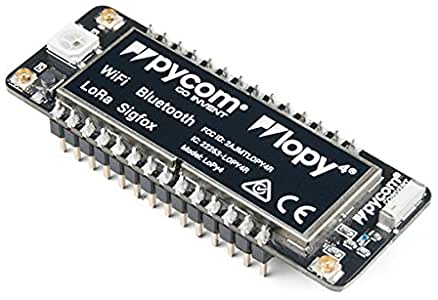
\includegraphics[width=.5\columnwidth]{Pictures/LoPy.jpg}  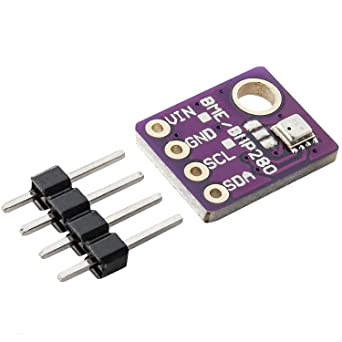
\includegraphics[width=.3\columnwidth]{Pictures/BME280.jpeg}}
\caption{LoPY4 et capteur BME280}
\label{fig-lopy-bme280}
\end{figure}

Un LoPY4 se programme en Python (ou plutôt \Index{micro-python} qui est la version du langage pour systèmes embarqués) pour traiter les données. Dans un premier temps, nous allons utiliser le Wi-Fi pour communiquer avec votre ordinateur mais, par la suite, nous mettrons en place une communication via \Index{LoRaWAN} ou \Index{Sigfox} qui peut vous demander plus de configuration mais vous permettra de mieux comprendre ces protocoles.

     \vspace{1em}


Même si vous n’avez pas de LoPy4, vous pouvez parcourir cette section pour voir les contraintes supplémentaires liées aux objets connectés.

\section{Installation d'Atom}

\Index{Atom} est un éditeur de texte performant, spécifiquement conçu pour le codage en différents langages. 
Atom va nous aider à programmer en Python et va également gérer la communication avec notre LoPy via le port \Index{USB} (grâce au plugin \Index{pymakr}). 
Atom fonctionne à peu près de la même manière sur \Index{Mac OS}, \Index{Windows} et \Index{Linux}, mais en s’adaptant aux particularités du système d’exploitation (place dans les menus, nom des liens séries...). 
Donc, il se peut que vous ayez quelques différences entre ce que vous avez dans cet ouvrage et l’écran de votre ordinateur. 
Les menus et sites Web indiqués peuvent également changer au cours du temps même si nous nous efforçons de faire des mises à jour régulières du cours.


     \vspace{1em}

Pour commencer à programmer avec votre LoPy, vous devez installer sur votre ordinateur le logiciel Atom (voir sur \url{http://atom.io}). 
Vous pouvez télécharger le package correspondant à votre système d'exploitation (cf. figure suivante).

\begin{figure}[tbp]
\centerline{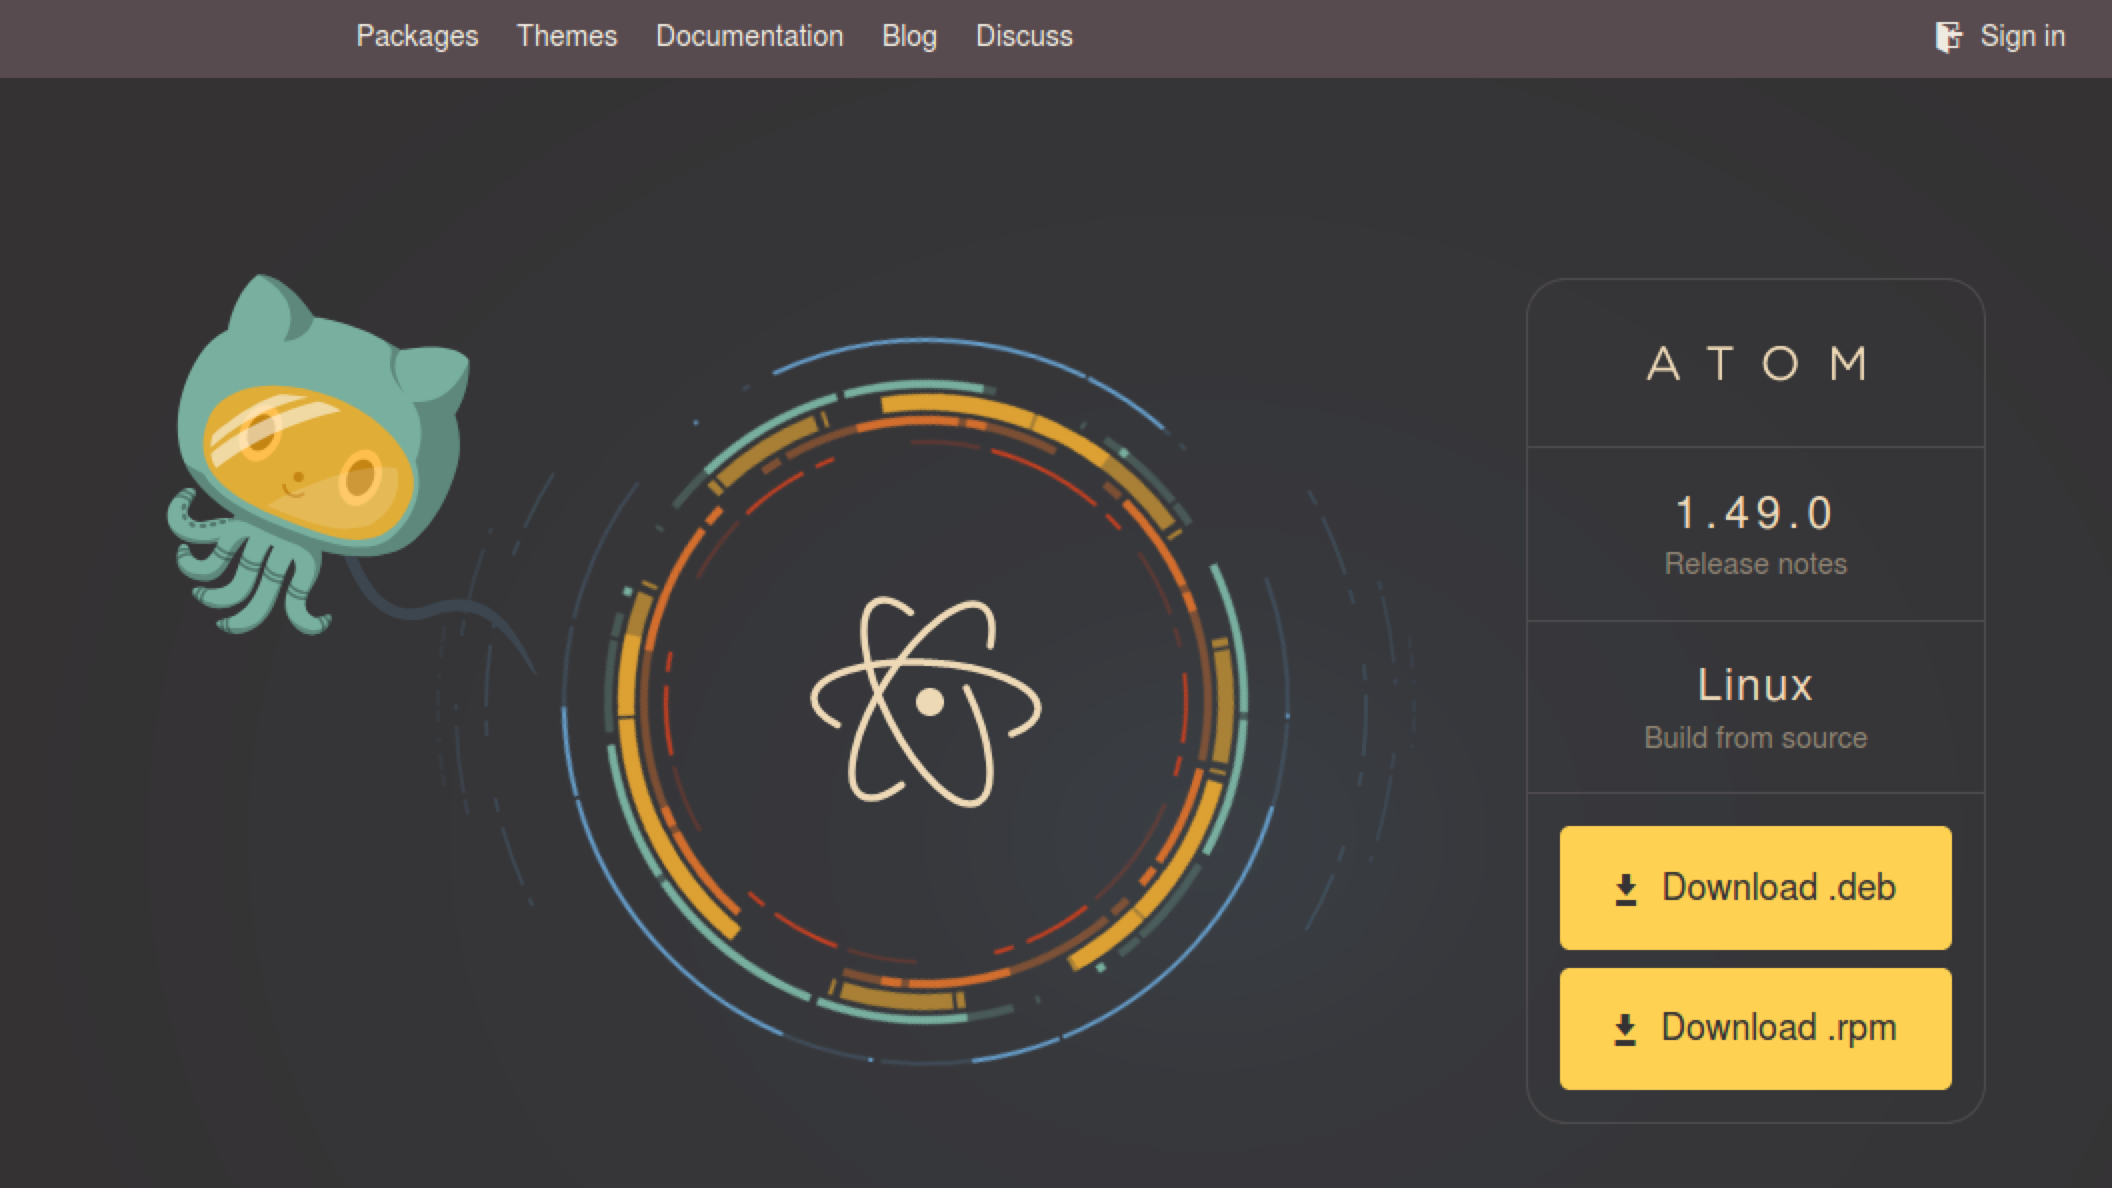
\includegraphics[width=1\columnwidth]{Pictures/atom_dl.png}}
\caption{Page d'accueil d'Atom}
\label{fig-page-atom}
\end{figure}
\begin{itemize}
\item Pour Mac et Windows, cliquez sur l’icône "télécharger" pour l’installer\footnote{il y a des risques d'incompatibilité des dernières versions d'Atom avec le package de gestion du LoPy (pymakr). Nous vous recommandons d'utiliser une version plus ancienne, comme la 1.43 disponible dans les archives d'Atom Release \url{https://github.com/atom/atom/releases/tag/v1.43.0}(\texttt{AtomSetup-x64.exe} pour Windows ou \texttt{atom-mac.zip} pour Mac OS).}.
\item Pour Linux, téléchargez le\texttt{.deb} et tapez \texttt{sudo dpkg -i atom-amd64.deb}\footnote{Il est possible qu'un message vous dise que git n'est pas installé. Dans ce cas, tapez \texttt{sudo apt-get install git} et suivez les instructions).}.
Lancez Atom en cliquant sur l’icône ou, sous Linux, en tapant atom dans un terminal.
\end{itemize}

     \vspace{1em}

Lancez Atom en cliquant sur l’icône ou, sous Linux, en tapant atom dans un terminal. L’écran d’accueil apparaît.

\subsection{Communiquez avec votre Pycom}

Pour communiquer avec le Pycom à travers Atom, vous devez installer le package pymakr.

Cliquez sur \textit{Install a Package} puis \textit{Open Installer}. Une autre fenêtre s’ouvre (cf. figure~\vref{fig-page-pakage}. Tapez \texttt{pymakr} dans le menu. Un package apparaît portant ce nom. Cliquez sur \textit{Install}. L’installation peut prendre plusieurs minutes. Vous avez le temps de prendre un café.

\begin{figure}[tbp]
\centerline{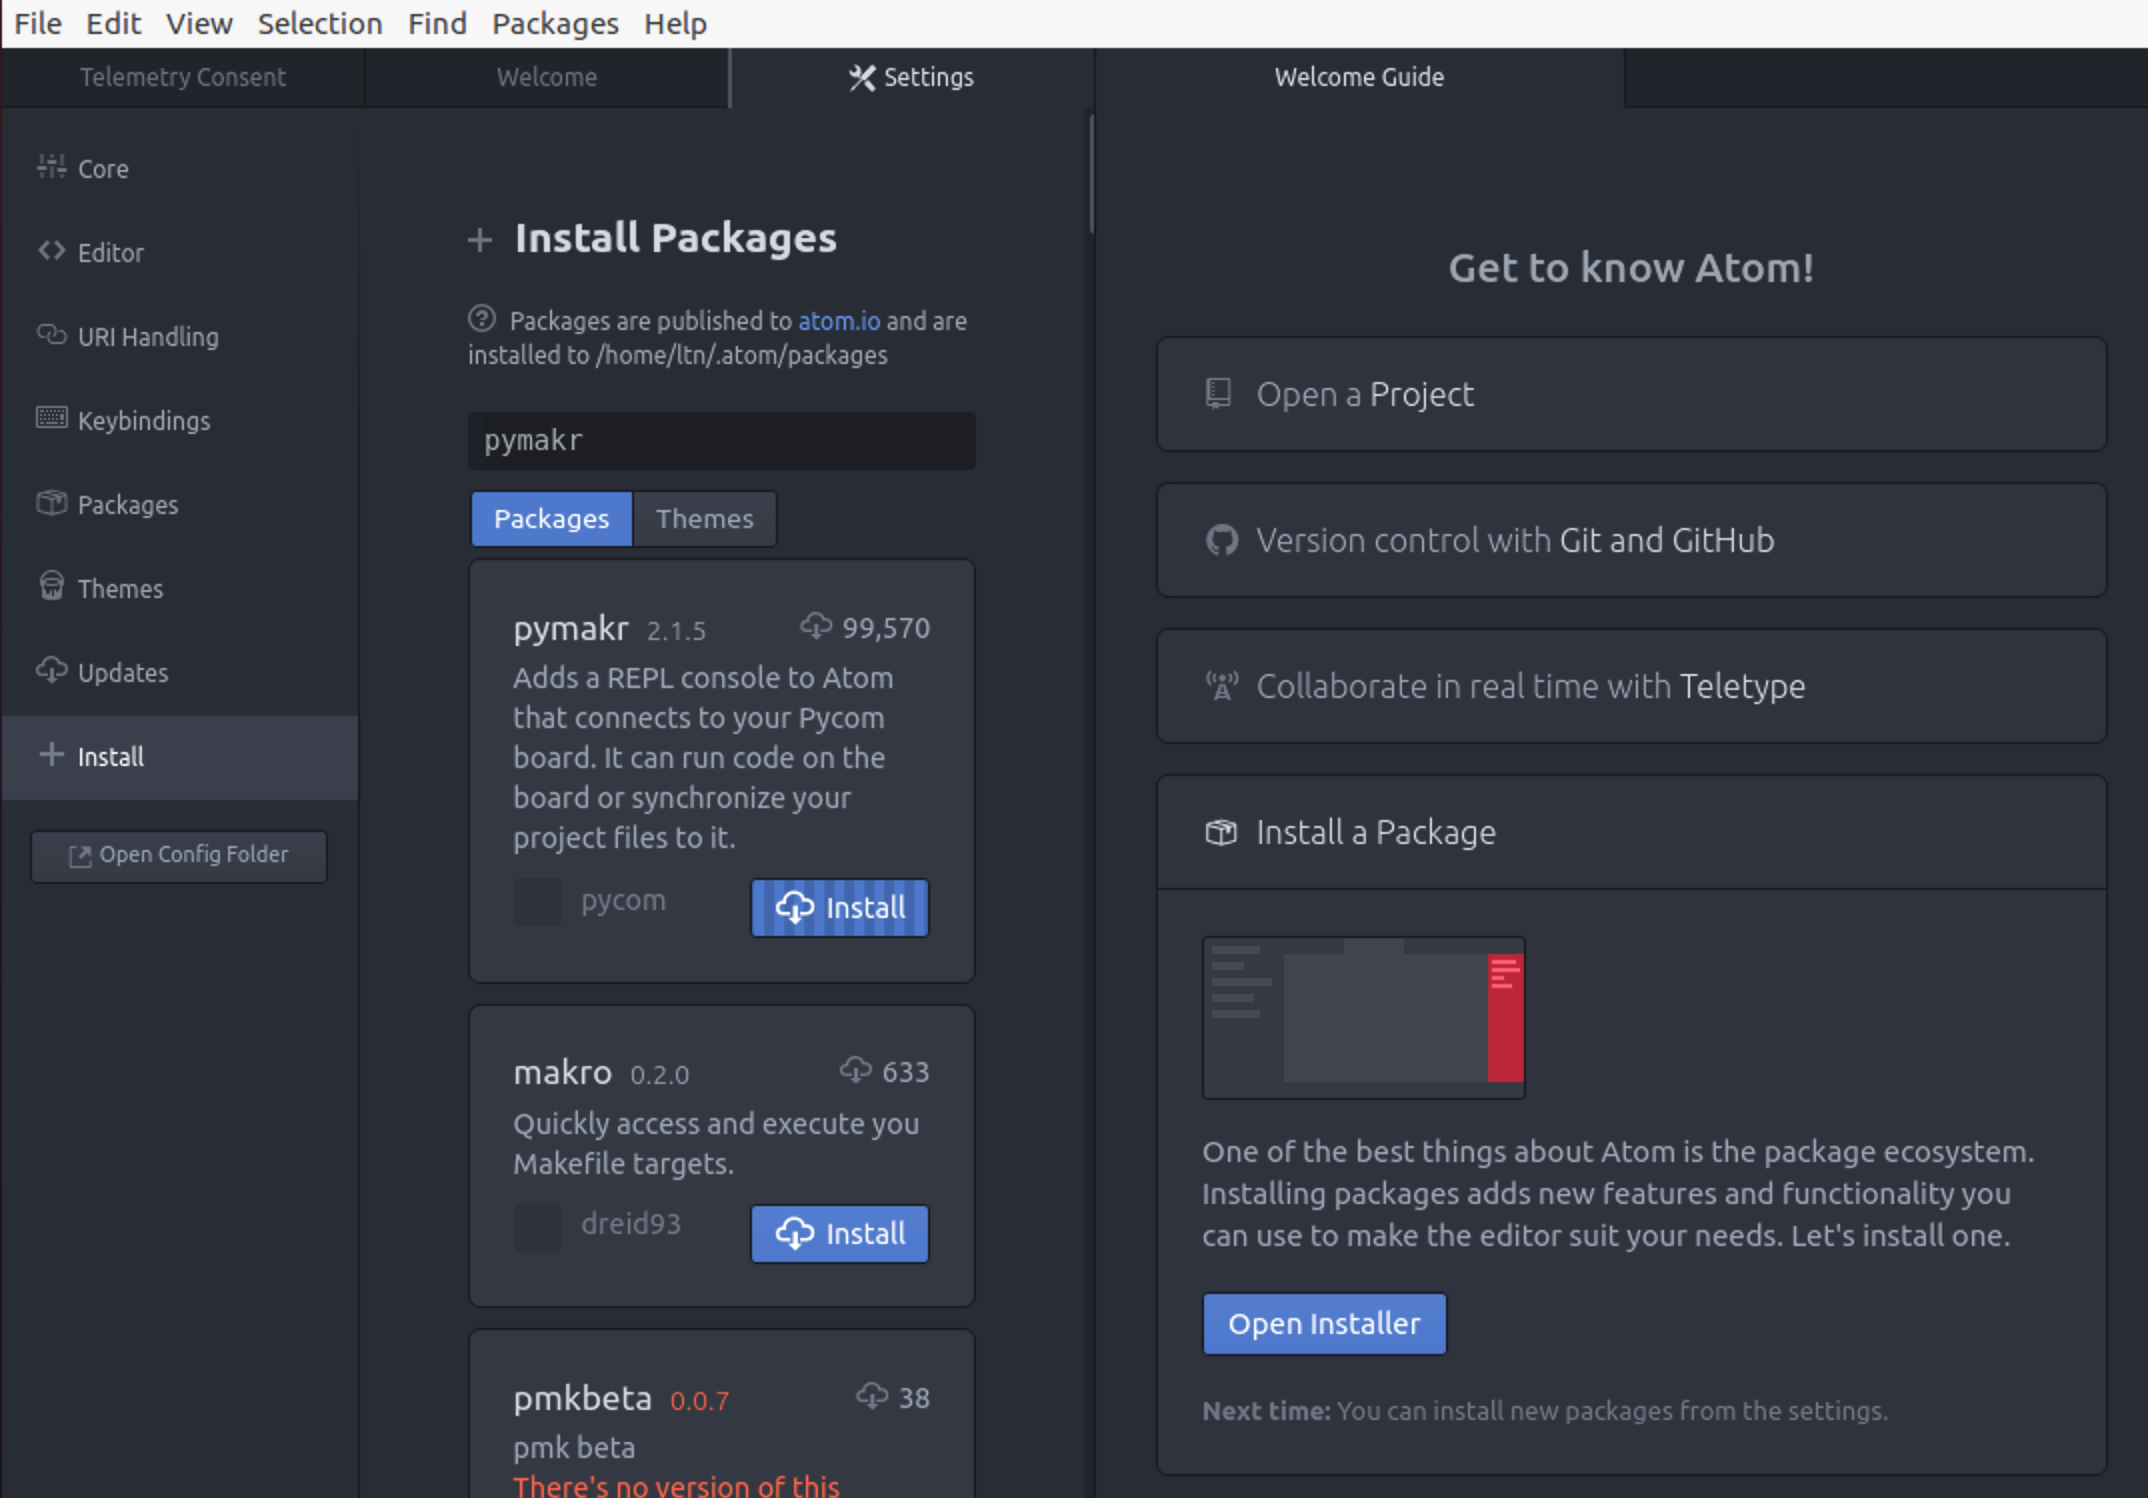
\includegraphics[width=1\columnwidth]{Pictures/atom_pymakr.png}}
\caption{Installation de Paquetages}
\label{fig-page-pakage}
\end{figure}

     \vspace{1em}

Une fois le café bu et l’installation terminée, une nouvelle fenêtre (terminal) s’ouvre en bas d’Atom.

     \vspace{1em}

Ce terminal (cf.figure~\vref{fig-page-pymakr}) vous permettra de dialoguer avec le LoPy.
Branchez le LoPy à votre ordinateur.
Vous devriez voir l’invite\texttt{ >{}>{}>{}} caractéristique d’un interpréteur Python\footnote{Sous Linux, vous devez être membre du groupe dialout pour pouvoir gérer la communication sur le port USB. 
Si vous ne voyez par l’invite, tapez \texttt{sudo adduser \textit{login} dialout} en remplaçant login par le nom de votre compte Linux. Reconnectez-vous sous votre compte.}.

     \vspace{1em}

\begin{figure}[tbp]
\centerline{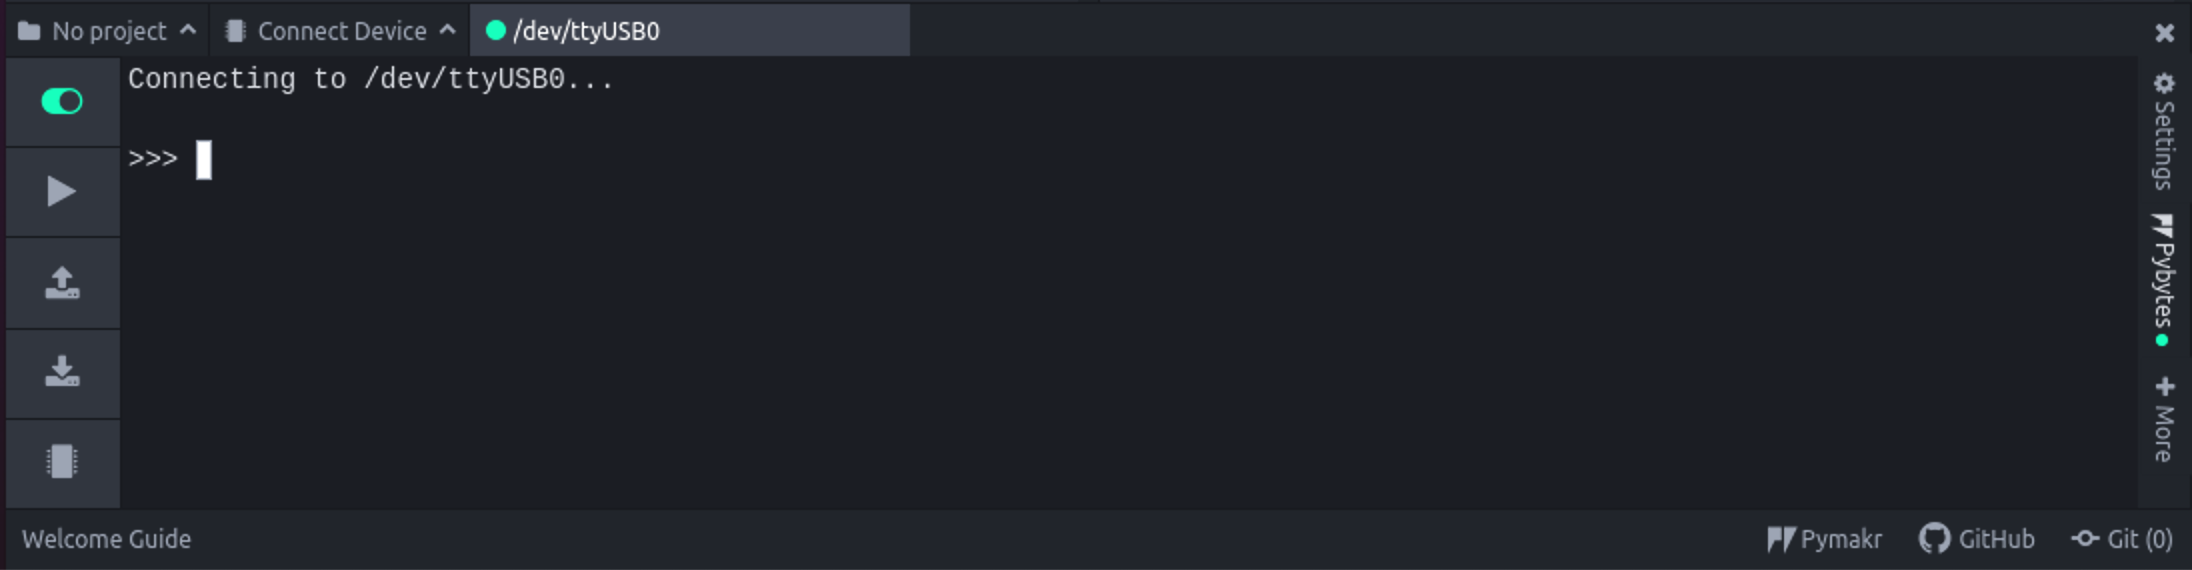
\includegraphics[width=1\columnwidth]{Pictures/atom_pymakr1.png}}
\caption{Fenêtre Pymakr}
\label{fig-page-pymakr}
\end{figure}

Toutes les commandes que vous allez taper dans cette fenêtre vont s’exécuter sur votre LoPy. Par exemple, si vous tapez\footnote{Les fenêtres sur fond gris montrent le code micropython et leur résultat.}~:

\begin{termc}[backgroundcolor=\color{gray!10}, basicstyle=\ttfamily\small, escapechar=@]
Connecting to /dev/ttyUSB0...
>>> @\textbf{1+1}@
2
>>>
\end{termc}

L’addition se fait sur le LoPy.

     \vspace{1em}

Sur le coté gauche de la fenêtre pymakr, plusieurs icônes sont présentes~:
\begin{itemize}
    \item l'interrupteur permet d'activer ou de désactiver le connexion avec le LoPy~;
    \item le triangle permet d'exécuter le programme affiché dans la fenêtre d'Atom sur le LoPy~;
    \item la flèche vers le haut, permet de recopier le répertoire actif dans la mémoire du LoPy. Cela sera utile pour installer de nouveaux modules sur le LoPy~;
    \item inversement le flèche vers le bas, permet de recopier la mémoire du LoPy sur l'ordinateur~;
    \item le processeur permet d'avoir des informations sur le loPy.
\end{itemize}

     \vspace{1em}

Sur la partie droite, l'onglet vertical \textit{Setting} permet de modifier les paramètres de connexion avec le LoPy.

\subsection{Installez votre environnement de travail} 

Pour programmer le LoPy, il faut récupérer les modules micropython. Le dépôt ca être téléchargé dans le répertoire de votre choix :

\begin{termc}[backgroundcolor=\color{gray!10},  basicstyle=\ttfamily\small, escapechar=@]
> git clone https://github.com/ltn22/PLIDObis.git
\end{termc}

Dans le menu \textit{Files>Open Folder} d’Atom, sélectionnez le répertoire \texttt{pycom} du dépot téléchargé, et validez. Sur la partie gauche de l’écran, l’ensemble des fichiers composant ce répertoire apparaissent. Il y en a beaucoup, car ils vont nous servir par la suite.

     \vspace{1em}

En cliquant dans la fenêtre \textit{\Index{pymakr}} sur le bouton \textit{Upload project to device}, les fichiers de ce répertoire vont être copiés dans la mémoire du LoPy. 
Par la suite, si un module est modifié, il devra être resynchronisé dans la mémoire du LoPy.

\section{Connexion au réseau Wi-Fi}

\begin{wrapfigure}{r}{3cm}
\Youtube{https://youtu.be/PmvSU8AWO68}
\end{wrapfigure}


Pour rattacher de LoPY à un réseau \Index{Wi-Fi}, il doit dans un premier temps être configuré via la liaison USB de l'ordinateur pour lui donner les paramètres nécessaires à la connexion. 


Le fichier \texttt{\Index{boot.py}} a été copié lors du téléversement des fichiers dans la mémoire du LoPy. Au démarrage du LoPy, ce programme va chercher à se connecte à un réseau Wi-Fi. Comme le nom du réseau et la clé sécrète n'ont pas été founie, il n’y arrive pas. Le LoPy se transforme  en point d’accès. Au démarrage, le LoPy a dû afficher le message suivant, indiquant que le LoPy devient point d'accès Wi-Fi et va déployer son propre réseau sur lequel votre ordinateur peut se connecter. Le nom de ce réseau de les la forme \texttt{PLIDO\_XXXX} où \texttt{XXXX} est une séquence hexadécimal propre à l'équipement. La clé est \texttt{www.pycom.io}. Le LoPy à l'adresse \texttt{192.168.4.1} sur ce réseau.  

\begin{termc}[backgroundcolor=\color{gray!10},  basicstyle=\ttfamily\small, escapechar=@]
Failed to connect to any known network, going into AP mode
To connect look for 'PLIDO_5bac' access point, key = 'www.pycom.io'
\end{termc}

Mais ce n'est pas très intéressant car votre ordinateur va perdre sa connexion à l'internet. Pas très pratique pour suivre le MOOC. Avant d'afficher ce message, le LopY a montré la liste des réseaux Wi-Fi qu'il a détecté. Vous pouvez à l'inverse le connecter à un de ces réseau en renseignant le fichier \texttt{wifi\_conf.py} qui se trouve dans le répertoire \texttt{pycom}.


\pycomlst{wifi\_conf.py}

\texttt{MON\_SSID} doit être remplacé par le nom du réseau Wi-Fi ou \ac{SSID} et \texttt{MON\_MOT\_DE\_PASSE} par la clé qui y est associée. Notez que plusieurs réseaux Wi-Fi peuvent être ajouté, puisque \texttt{MON\_SSID} est vu comme une clé de l'objet JSON. L'édition de fichier s'est faite sur l'ordinateur, il doit être recopié dans la mémoire du LoPy en cliquant sur la flèche vers le haut.

Le Pycom redémarre et doit maintenant afficher un message du genre :

\begin{termc}[backgroundcolor=\color{gray!10}, basicstyle=\ttfamily\small, escapechar=@]
net to use ['MONWIFI']
Connected to MONWIFI with IP address: @\ul{192.168.1.76}@
Pycom MicroPython 1.20.2.r1 [v1.11-a5aa0b8] on 2020-09-09; LoPy4 with ESP32
Type "help()" for more information.
>>> 
\end{termc}



Il est possible de pinguer ou de se connecter avec \Index{FTP} ou \Index{telnet} en utilisant cette adresse IP.

\begin{termc}[backgroundcolor=\color{palerod},  basicstyle=\ttfamily\small, escapechar=@]
# @\textbf{telnet \ul{192.168.1.76}}@
Trying 192.168.1.86...
Connected to 192.168.1.86.
Escape character is '^]'.
MicroPython v1.8.6-760-g90b72952 on 2017-09-01; LoPy with ESP32
Login as: micro
Password: python
Login succeeded!
Type "help()" for more information.
>>>
\end{termc}


Ça peut être utile pour suivre le comportement de votre objet sans lancer atom si l'objet n'est plus connecté via la liaison USB à l'ordinateur. 

Atom peut également être configuré pour utiliser cette adresse IP. La configuration se fait dans le menu \textit{setting}, et en entrant l'adresse ip du LoPy et en désactivant \textit{auto connect}. Au prochain lancement d'Atom, il sera possible joindre le LoPy en Wi-Fi.


\section{Mise en place d'un client}

\begin{wrapfigure}{r}{3cm}
\Youtube{https://youtu.be/Mi3e4c2E59o}
\end{wrapfigure}


Un programme relativement simple permet de vérifier la communication entre le LoPy et le serveur. La commande \Index{ifconfig}\footnote{Sous Linux, il faut ajouter le paquetage \Index{net-tools} \texttt{sudo apt install net-tools}.} donne l'adresse IP du serveur. L'adresse doit être différente de celle que l'on avait obtenu sur le LoPy. 

Si le serveur tourne dans un environnement local, l'adresse devrait commencer par \texttt{192.168} ou \texttt{10}. Si le LoPy et l'ordinateur sont connectés au même réseau Wi-Fi, les premiers chiffres doivent être identiques. 

Si le serveur tourne sur un serveur à l'extérieur (i.e. le \textit{cloud}), l'adresse est quelconque.

     \vspace{1em}

La commande suivante est tapée depuis le terminal de l'ordinateur, on remarque les deux interfaces disponibles l'une pour le réseau Ethernet ou Wi-Fi et l'une pour le \textit{\Index{loopback}}, les noms des interfaces peuvent changer d'une configuration à une autre~:

\begin{termc}[backgroundcolor=\color{palerod},  basicstyle=\ttfamily\small, escapechar=@]
> @\textbf{ifconfig}@
eth1      Link encap:Ethernet  HWaddr 10:65:30:b0:54:bf
          inet addr:@\ul{192.168.1.237}@  Bcast:192.168.1.255  Mask:255.255.255.0
          inet6 addr: fe80::d8ac:86e7:8bdb:e333/64 Scope:Unknown
          UP BROADCAST RUNNING MULTICAST  MTU:1500  Metric:1
          RX packets:0 errors:0 dropped:0 overruns:0 frame:0
          TX packets:0 errors:0 dropped:0 overruns:0 carrier:0
          collisions:0
          RX bytes:0 (0.0 B)  TX bytes:0 (0.0 B)

lo        Link encap:Local Loopback
          inet addr:127.0.0.1  Mask:255.0.0.0
          inet6 addr: ::1/128 Scope:Unknown
          UP LOOPBACK RUNNING  MTU:1500  Metric:1
          RX packets:0 errors:0 dropped:0 overruns:0 frame:0
          TX packets:0 errors:0 dropped:0 overruns:0 carrier:0
          collisions:0
          RX bytes:0 (0.0 B)  TX bytes:0 (0.0 B)
\end{termc}

Le programme \pprog{minimal\_server.py}{plido-tp3} présenté au chapitre~\vref{chap-mini-serv} n'a pas été modifié et attend des données sur le port 33033.

     \vspace{1em}

\pycomlst{sending\_client.py}

Le programme \lprog{sending\_client.py}{pycom} doit être modifié (ligne 4) pour prendre en compte l'adresse IP du serveur obtenue avec la commande \texttt{ifconfig}. Si à chaque exécution sur le LoPy de ce programme, le serveur reçoit la valeur, la communication est établie entre les deux équipements.

\begin{termc}[backgroundcolor=\color{palerod}, basicstyle=\ttfamily\small, escapechar=@]
> @\textbf{python3 minimal\_server.py}@
b'message' => b'6d657373616765'
b'message' => b'6d657373616765'
\end{termc}


\section{BME 280}

\begin{wrapfigure}{r}{3cm}
\Youtube{https://youtu.be/I3zc3-qoq2s}
\end{wrapfigure}

Au lieu de générer de fausses données, nous allons dans cette section utiliser un vrai capteur de température humidité pression : le BME 280 de chez Bosch. 


\subsection{Le bus I2C}

Le bus I2C est  normalisé par le fabricant de composants électroniques  \Index{NXP}\footnote{\url{https://www.nxp.com/docs/en/user-guide/UM10204.pdf}} ce qui permet une meilleure interopérabilité entre les composants.

 \begin{figure}[!ht] 
\centering 


	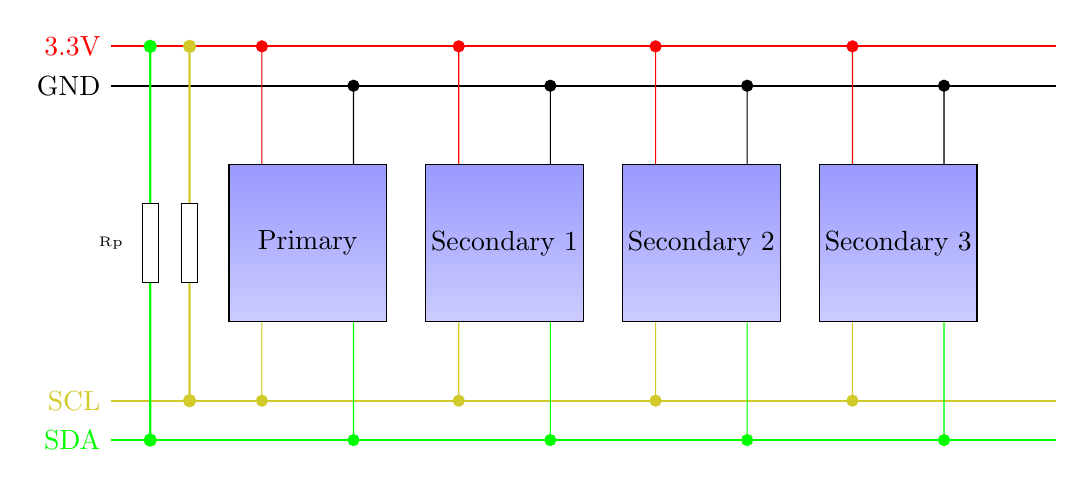
\begin{tikzpicture}
	
	\draw [thick, red] (0, 7.5) node [left] {3.3V} coordinate (l1) -- +(12, 0); 
	\draw [thick, black] (0, 7) node [left] {GND} coordinate (l2) -- +(12, 0); 
	
	\draw [thick, yellow!80!black] (0, 3) node [left] {SCL} coordinate (l3) -- +(12, 0); 
	\draw [thick, green] (0, 2.5) node [left] {SDA} coordinate (l4) -- +(12, 0); 
	
	\foreach \i/\n in {1/Primary, 2/Secondary 1, 3/Secondary 2, 4/Secondary 3} {
		\draw (2.5*\i, 5) node (n\i) [rectangle, top color=blue!40, bottom color=blue!20, draw, minimum size= 2cm]{};
		
		\draw (n\i) node {\n};
		
		\filldraw [red] (n\i.120) -- (n\i.120 |-l1) circle  (2pt);
		\filldraw [black] (n\i.60) -- (n\i.60 |-l2) circle  (2pt);
		\filldraw [yellow!80!black] (n\i.-120) -- (n\i.-120 |-l3) circle  (2pt);
		\filldraw [green] (n\i.-60) -- (n\i.-60 |-l4) circle  (2pt);
	}

	\coordinate (v1) at (0.5, 0);
	\coordinate (v2) at (1, 0);
	
	\filldraw [thick, green] (v1 |- l1) circle  (2pt) -- coordinate (r1) (v1 |- l4)circle  (2pt);
	\filldraw [thick, yellow!80!black] (v2 |- l1)circle  (2pt) -- coordinate (r2) (v2 |- l3)circle  (2pt);
	
	\filldraw [white]  ([xshift=-0.1cm, yshift=-0.5cm]r1) rectangle ++(0.2, 1); 
	\draw ([xshift=-0.1cm, yshift=-0.5cm]r1) rectangle ++(0.2, 1); 
	
	\draw  ([xshift=-0.5cm]r1) node {\tiny{Rp}};
	
	\filldraw [white] ([xshift=-0.1cm, yshift=-0.5cm]r1-|r2) rectangle ++(0.2, 1); 
	\draw ([xshift=-0.1cm, yshift=-0.5cm]r1-|r2) rectangle ++(0.2, 1); 
	
	

	\end{tikzpicture}
\caption{bus I2C} 
\label{fig-busI2C} 
\end{figure} 	

Sur un des fils le signal d'horloge va être émis par le primaire. Sur l'autre fil, les données seront codées soit dans le sens primaire/secondaire, soit dans l'autre. Comme avec \Index{Modbus}, les communications entre un secondaire et le primaire seront gérées par le primaire. 
Chaque secondaire est configuré avec une adresse unique sur le bus. Soit le maître envoie des données vers cette adresse\footnote{Il s'agit d'un abus de langage, en effet les données émises par le primaire sont reçues par l'ensemble des secondaires, mais seul celui qui est destinataire (i.e. qui reconnaît son adresse) va les traiter, les autres équipements ignoreront l'information.}, soit le primaire interroge l'esclave pour obtenir ses données. Le fil sera donc exploité dans les deux directions. 

La lecture de l'information binaire se fait lorsque le signal d'horloge est à l'état haut (cf. figure~\vref{fig-exI2C}). Quand le signal SDA est à l'état haut, un bit à 1 est transmis et dans l'état bas un bit à 0 est transmis.  Les changements d'état du signal SDA se font donc quand le signal d'horloge est à l'état bas. 

Il existe malgré tout deux exceptions~: si le signal SDA passe de l'état haut à l'état bas tandis que le signal d'horloge est à l'état haut cela indique un début de transmission de données. Si le signal SDA passe de l'état bas à l'état haut dans les mêmes conditions, cela indique la fin de transmission de données. Entre les deux les données binaires forment une trame (ou un PDU dans le vocabulaire ISO) qui est structuré comme indiqué figure~\vref{fig-exI2C}.


  \begin{figure}[!ht] 
\centering 
 \pgfdeclarelayer{foreground}
 \pgfdeclarelayer{background}

\begin{tikztimingtable} [timing/d/background/.style={fill=white}, timing/lslope=0.2]
            SDA & H H L L L 4D 4D; [dotted] 4D; 4D 4D  LLLL HHHH\\
            SCL & HHHH 2T 2T 2T 2T 2T; [dotted] 2T; 2T 2T 2T 2T 2T HHHHHH \\
 \extracode
 % Add vertical lines in two colors
  \begin{pgfonlayer}{background}
    \begin{scope}[semitransparent,semithick]
      \draw   (2.2, 1.2) node (S) [below, rectangle, draw, minimum width=0.4cm,minimum height=1.2cm, pattern=dots, pattern color=purple]{};
      \draw (S.south) node [below] {S};
      
      \draw   (29, 1.2) node (P) [below, rectangle, draw, minimum width=0.4cm,minimum height=1.2cm, pattern=dots, pattern color=purple]{};
      \draw (P.south) node [below] {P};
      
     \foreach \i in {7.1,11.1,...,23.1} {
       \draw   (\i, 1.2) node (B) [below, rectangle, draw, minimum width=0.4cm,minimum height=1.2cm, color=purple]{};
        \draw (B.south) node [below] {0/1};
  
     }


    \end{scope}
  \end{pgfonlayer}
 
 \end{tikztimingtable}%


\caption{Exemple de communication avec le bus I2C} 
\label{fig-exI2C} 
\end{figure}

La figure~\vref{fig-tramesI2C} donne les formats les plus utilisés. 

\begin{figure}[!ht] 
\centering 
\begin{tikzpicture}

	\draw (0,0) node (S) [rectangle, draw, pattern=dots, pattern color=purple, minimum width=0.3cm, minimum height=0.5cm]{};
	\draw (S) node {\tiny{S}};  
	
	\coordinate (a) at (S.east);
	\foreach \i in {7,...,1}{
 		\draw (a) node (A\i) [right, rectangle, draw, fill=purple, minimum width=0.3cm, minimum height=0.5cm]{};
 		\draw (A\i) node [text width=0.3cm, text centered] {\tiny{A\\\i\\}};
 		
 		\coordinate (a) at (A\i.east);	
	}
 	\draw (a) node (RW) [right, rectangle, draw, fill=purple, minimum width=0.3cm, minimum height=0.5cm]{};
 	\draw (RW) node [text width=0.3cm, text centered] {\tiny{0\\}};


 	\draw (RW.east) node (Ack1) [right, rectangle, draw, fill=yellow, minimum width=0.3cm, minimum height=0.5cm]{};
 	\draw (Ack1) node [text width=0.3cm, text centered] {\fontsize{6}{4}{\selectfont a\\c\\k\\}};
 	
 	\coordinate (a) at (Ack1.east);
	\foreach \i in {8,...,1}{
 		\draw (a) node (D1-\i) [right, rectangle, draw, fill=purple, minimum width=0.3cm, minimum height=0.5cm]{};
 		\draw (D1-\i) node [text width=0.3cm, text centered] {\tiny{D\\\i\\}};
 		
 		\coordinate (a) at (D1-\i.east);	
	}
 	\draw (a) node (Ack2) [right, rectangle, draw, fill=yellow, minimum width=0.3cm, minimum height=0.5cm]{};
 	\draw (Ack2) node [text width=0.3cm, text centered] {\fontsize{6}{4}{\selectfont a\\c\\k\\}};

 	\draw [dashed] (Ack2) -- ++(1, 0) coordinate (a);
	\foreach \i in {8,...,1}{
 		\draw (a) node (D2-\i) [right, rectangle, draw, fill=purple, minimum width=0.3cm, minimum height=0.5cm]{};
 		\draw (D2-\i) node [text width=0.3cm, text centered] {\tiny{D\\\i\\}};
 		
 		\coordinate (a) at (D2-\i.east);	
	}
 	\draw (a) node (Ack3) [right, rectangle, draw, fill=yellow, minimum width=0.3cm, minimum height=0.5cm]{};
 	\draw (Ack3) node [text width=0.3cm, text centered] {\fontsize{6}{4}{\selectfont a\\c\\k\\}};
	
	\draw (Ack3.east) node (P) [right, rectangle, draw, pattern=dots, pattern color=purple, minimum width=0.3cm, minimum height=0.5cm]{};
	\draw (P) node {\tiny{P}};  


	\draw (0,-1) node (S) [rectangle, draw, pattern=dots, pattern color=purple, minimum width=0.3cm, minimum height=0.5cm]{};
	\draw (S) node {\tiny{S}};  
	
	\coordinate (a) at (S.east);
	\foreach \i in {7,...,1}{
 		\draw (a) node (A\i) [right, rectangle, draw, fill=purple, minimum width=0.3cm, minimum height=0.5cm]{};
 		\draw (A\i) node [text width=0.3cm, text centered] {\tiny{A\\\i\\}};
 		
 		\coordinate (a) at (A\i.east);	
	}
 	\draw (a) node (RW) [right, rectangle, draw, fill=purple, minimum width=0.3cm, minimum height=0.5cm]{};
 	\draw (RW) node [text width=0.3cm, text centered] {\tiny{1\\}};


 	\draw (RW.east) node (Ack1) [right, rectangle, draw, fill=yellow, minimum width=0.3cm, minimum height=0.5cm]{};
 	\draw (Ack1) node [text width=0.3cm, text centered] {\fontsize{6}{4}{\selectfont a\\c\\k\\}};
 	
 	\coordinate (a) at (Ack1.east);
	\foreach \i in {8,...,1}{
 		\draw (a) node (D1-\i) [right, rectangle, draw, fill=yellow, minimum width=0.3cm, minimum height=0.5cm]{};
 		\draw (D1-\i) node [text width=0.3cm, text centered] {\tiny{D\\\i\\}};
 		
 		\coordinate (a) at (D1-\i.east);	
	}
 	\draw (a) node (Ack2) [right, rectangle, draw, fill=purple, minimum width=0.3cm, minimum height=0.5cm]{};
 	\draw (Ack2) node [text width=0.3cm, text centered] {\fontsize{6}{4}{\selectfont a\\c\\k\\}};
 	
 	\draw [dashed] (Ack2) -- ++(1, 0) coordinate (a);

	\foreach \i in {8,...,1}{
 		\draw (a) node (D2-\i) [right, rectangle, draw, fill=yellow, minimum width=0.3cm, minimum height=0.5cm]{};
 		\draw (D2-\i) node [text width=0.3cm, text centered] {\tiny{D\\\i\\}};
 		
 		\coordinate (a) at (D2-\i.east);	
	}
 	\draw (a) node (Ack3) [right, rectangle, draw, fill=purple, minimum width=0.3cm, minimum height=0.5cm]{};
 	\draw (Ack3) node [text width=0.3cm, text centered] {\fontsize{6}{4}{\selectfont a\\c\\k\\}};
	
	\draw (Ack3.east) node (P) [right, rectangle, draw, pattern=dots, pattern color=purple, minimum width=0.3cm, minimum height=0.5cm]{};
	\draw (P) node {\tiny{P}};  

\end{tikzpicture}


\caption{Exemple de communication avec le bus I2C} 
\label{fig-tramesI2C} 
\end{figure} 

Le premier train binaire illustre la transmission de données du primaire vers un secondaire. Le primaire commence par émettre un signal non binaire (\texttt{S}) indiquant un début de transmission. Les 7 bits suivants donnent l'adresse du secondaire et le bit suivant indique si le primaire veut envoyer des données (valeur à \texttt{0}) ou recevoir des informations du secondaire (valeur à \texttt{1}). 

Si un secondaire reconnaît son adresse sur le bus, alors il écrit le bit suivant dans le train binaire. Le primaire est donc informé en lisant cette valeur que le secondaire est bien présent sur le bus et qu'il peut recevoir des données. Le primaire va donc les envoyer octet par octet. Chaque octet étant acquitté de la même manière par le secondaire. Le train binaire se termine par le signal non binaire (\texttt{P}).

Dans le cas où le primaire souhaite recevoir, une fois le bit de début et les bits de l'adresse émis, le huitième bit est positionné à 1. Le secondaire acquitte puis transmet ses octets que le primaire acquitte.

\Question{scan}
{Le module I2C du LoPy dispose d'une fonction \pfunction{machine}{scan} qui affiche les adresses des secondaires connectés. Comment cette détection est possible ?}
{Le primaire va tester toutes les adresses possibles et y envoyer une trame, si le bit suivant l'adresse dans la trame n'est pas positionné par le secondaire, il n'y a aucun équipement connecté à cette adresse.}

\Question{Diffusion}{
Est-ce que la norme une adresse qui permet de parler à tous les secondaires en même temps ? }
{La norme prévoit un \textit{General Call} pour joindre tous les secondaires en utilisant l'adresse 0 (voir chapitre 3.1.12 du standard I2C)}


\subsection {Mesure de la température}

La communication entre le LoPy et le composant se fait via le bus \Index{I2C}. Il nous faut donc quatre fils pour le relier (cf. figure~\vref{fig-lopy-bme280-i2c}~: 
\begin{itemize}
    \item la masse (\texttt{\Index{GND}}), 
    \item une alimentation électrique de 3.3v (\texttt{\Index{VIN}}), 
    \item un fils pour l'horloge (\texttt{\Index{SCL}}) et 
    \item un autre finalement pour les données (\texttt{\Index{SDA}}).
\end{itemize} 

\begin{figure}[tbp]
\centerline{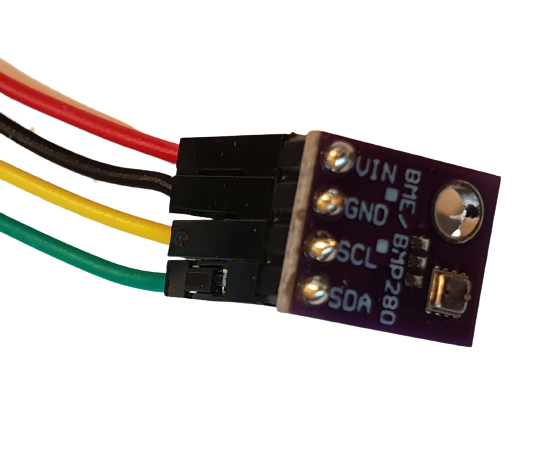
\includegraphics[width=.5\columnwidth]{Pictures/BME280-i2c.png}  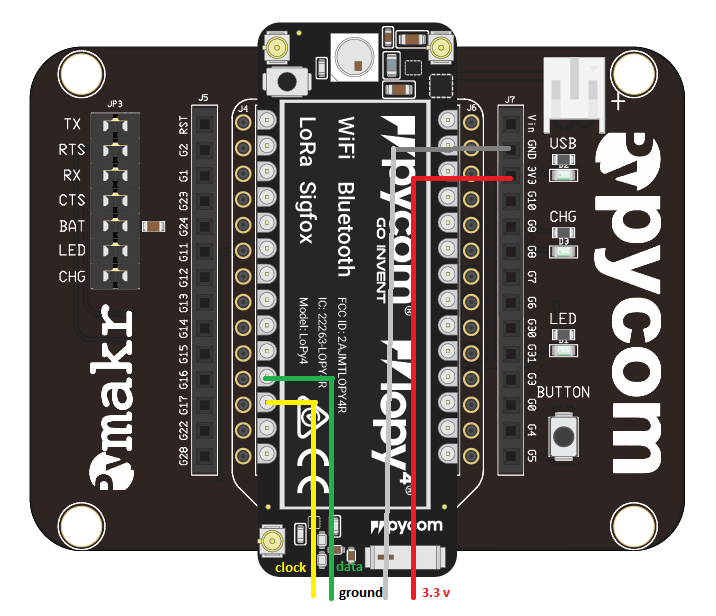
\includegraphics[width=.5\columnwidth]{Pictures/LoPy4.png}  }
\caption{capteur BME280 et connecteurs}
\label{fig-lopy-bme280-i2c}
\end{figure}

     \vspace{1em}

Pour ce faire, il faut connecter:
~\begin{itemize}
    \item la masse GND du LoPy sur la broche GND du composant avec un fil noir,
    \item l’alimentation en 3.3V du LoPy (3V3) sur VIN du composant avec un fil rouge (ce port s’appelle également \Index{DCC} sur certaines cartes),
    \item Le signal d’horloge du port G18/P10 du LoPy (ou G17 sur les versions LoPy 1) sur le port SCL du composant avec un fil jaune (ce port s’appelle également \Index{CLC} sur certaines cartes),
    \item Le fil de données du port G16/P9 du Pycom sur le port SDA du composant avec un fil vert.
\end{itemize}

Si le BME280 est connecté correctement sur les connecteurs du LoPy, vous devez obtenir le résultat suivant~:

\begin{termc}[backgroundcolor=\color{gray!10}, basicstyle=\ttfamily\tiny, escapechar=@]
>>> Running BME280.py

>>> 
>>> 
[118]
temp 550576 27.98  - hum 26626 48.784 % - pres 389338 pres 1004.494 hPa [delta -389338 ]
temp 551952 28.42  - hum 26587 48.557 % - pres 389712 pres 1004.527 hPa [delta -374 ]
temp 551792 28.37  - hum 26577 48.491 % - pres 389664 pres 1004.621 hPa [delta 48 ]
temp 551712 28.34  - hum 26594 48.596 % - pres 389648 pres 1004.654 hPa [delta 16 ]
temp 551632 28.32  - hum 26587 48.546 % - pres 389616 pres 1004.713 hPa [delta 32 ]
\end{termc}

Vous pouvez soit toucher le capteur, soit souffler dessus pour faire augmenter la température ou la pression.

     \vspace{1em}

\pycomlst[firstline=282, firstnumber=282]{BME280.py} %[firstline=282,lastline=19, firstnumber=282]

Le programme \lprog{BME280.py}{pycom} peut fonctionner comme un module mais la dernière partie donne un exemple d'exploiation des résultats~:

\begin{itemize}

\item Le programme principal commence par importer (ligne 283) le module gérant le bus I2C. Il est invoqué à la ligne 286. Le LoPy va gérer la communication avec le BME280, donc l’adresse est \texttt{0} et son statut est\texttt{MASTER}. La vitesse de communication est ensuite spécifiée.

\item La ligne suivante scanne le bus pour trouver des composants. Si tout va bien, il devrait en trouver un à l’adresse 118 qui correspond à  l’adresse par défaut du BME280\footnote{Si une autre valeur est indiquée, vous pouvez à l'instantiation du module BME280, ligne 289, ajouter le paramètre \texttt{addr=\textit{valeur}}. }. Sinon, revoyez votre câblage.

\item Le module BME280 est initialisé en lui passant en paramètre la référence du bus I2C précédemment défini.

\item Le programme va ensuite afficher les valeurs captées par le composant. Il existe deux types de valeurs : brutes (\textit{raw}) et calibrées. Les premières réagissent plus rapidement aux changements cependant sont beaucoup plus bruitées que les secondes qui subissent un traitement mathématique.

Ainsi, les première et deuxième colonnes donnent les températures brute et calibrée. On y accède par les méthodes \pfunction{BME280}{read\_raw\_temp} et \pfunction{BME280}{read\_temperature}. Il en va de même pour les deux autres grandeurs, humidité et pression.
\item Le programme affiche également l’écart de pression brute entre deux mesures. Cela permet de mettre plus facilement en évidence le fait que l’on souffle sur le capteur.
\end{itemize}

\section{Thermomètre Wi-Fi}

\begin{wrapfigure}{r}{3cm}
\Youtube{https://youtu.be/Ie-hGkkhsMQ}
\end{wrapfigure}

Vous avez maintenant tous les outils pour récupérer la température de votre logement, la transmettre à votre ordinateur via le Wi-Fi, et la transmettre à Beebotte pour l'afficher. Il y a très peu de changement par rapport à la version complètement sur ordinateur. Le programme de transformation de la structure CBOR de représentation des séries temporelles en JSON compréhensible par Beebottte reste le même. Il faudra juste modifier le nom du capteur d'humidité à température.

Le programme que vous avez construit lors du TP précédent utilisait le module \texttt{virtual\_sensor} pour produire des séries temporelles aléatoires symbolisant le comportement d'un capteur. Maintenant que nous avons un \Index{BME280}, nous allons pouvoir traiter de vraies valeurs.

     \vspace{1em}

Le programme \lprog{wifi\_temperature.py}{pycom} montre cette adaptation.

\pycomlst{wifi\_temperature.py}\label{prog-wifi-temp}

Au niveau des importations de modules, \texttt{BME280} et \texttt{\index{I2C}} remplacent \texttt{virtual\_sensor}, et le module \texttt{CBOR} est celui de \texttt{\Index{kpn\_senml}}. 
Mais son comportement reste le même, en particulier la fonction \pfunction{kpn\_senml}{dumps} qui convertit une structure Python en CBOR. Il vous reste à adapter la ligne 26 pour mettre l’adresse IP de votre ordinateur.

     \vspace{1em}

Côté ordinateur, vous devez relancer le programme \pprog{display\_server.py}{plido-tp3}, mais en modifiant le nom du capteur de "humidity" à "temperature". 

     \vspace{1em}

Sur votre compte Beebotte, au bout de 300 secondes, vous devez voir des données associées au capteur "temperature".

\Question{changement de pas}
{Que se passe-t-il si dans le programme \lprog{wifi\_temperature.py}{pycom} vous modifiez le pas de mesure ligne 36, pour le mettre par exemple à 60 secondes.}
{
Le programme \pprog{display\_server.py}{plido-tp3} doit être modifié également en ajoutant l'argument \texttt{period=60} à l'appel de \texttt{to\_bbt}.
}

